% -----------------------------------------------------------
\chapter{Introduction}
\label{sec:theory}
% -----------------------------------------------------------

Here is space for some general introduction.
The Standard Model (\SM) of elementary particles~%
\cite{Glashow:1961tr,Weinberg:1967tq,Salam:1968rm,Glashow:1970gm,Georgi:1972cj,Gross:1973id,Politzer:1973fx,tHooft:1971akt,tHooft:1971qjg,tHooft:1972tcz,tHooft:1972qbu}
is the best and most complete theory of elementary particles and their interactions to date.
An overview of all particles of the \SM is given in \cref{fig:sm-overview}.

The thesis is organised as follows.
\Cref{chap:results} presents the results, before a summary and conclusions are given in \cref{chap:conclusions}.

\begin{figure}
  \centering
  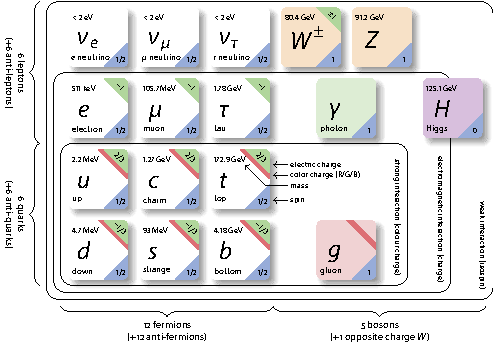
\includegraphics[width=0.86\textwidth]{figures/sm-overview}
  \caption[Particles of the Standard Model]{%
    The particles of the Standard Model.
    The quoted mass values are according to Ref.~\cite{PhysRevD.98.030001}.
    The code for this figure is available on github: \url{https://github.com/knutzk/sm-overview-figure}.
  }
  \label{fig:sm-overview}
\end{figure}


\section{Organisation of this template}

The idea of this template is simple: keep all the different chapters in individual tex files.
That makes the whole writing experience a lot cleaner and it's easier to find stuff.
I would also recommend starting a new line with each sentence, because that makes it easier to track changes in git sentence by sentence.
Tex files for the individual chapters are stored in the \texttt{tex/} subdirectory and then included into the main document with the \texttt{\textbackslash include\{tex/chapter\}} command.
You can use the \texttt{\textbackslash includeonly\{tex/chapter\}} command to switch off some of the chapters of the thesis (without breaking cross-references!).

Figures should go into their own directory, \texttt{figures/}.
And it's probably best to create subdirectories there for each chapter/topic to keep the figures organised in a way.

There are a few extra files to look out for:
%
\begin{itemize}
  \item \texttt{dissertation-defs.sty} -- define abbreviations, common symbols etc. here, and then use them consistently throughout the text. For example, you shouldn't always type \texttt{\$t\textbackslash bar\{t\}\$}, but instead you should pre-define a command such as \texttt{\textbackslash ttbar}. It's gonna make it easier to use these symbols consistently in the text and also makes your latex code much easier to read.
  \item \texttt{dissertation-bib.bib} -- this is where bibliography entries should go. Make sure that all necessary fields are given for each entry type, e.g. an article should always have an author, title, journal, volume, year and pages.
  \item \texttt{tex/abstract\_en/de.tex} -- there are two files for the thesis abstract: one for the English version, one for the German version. Whether you need both is up to you. My personal take is: if the thesis is written in English and the title page is already in English, then there's no need to include a German abstract at all. You should comment/uncomment the abstract files in the main document accordingly.
  \item \texttt{tex/title\_english/german.tex} -- this is where the title page is defined, either in English or in German. Make a choice and comment/uncomment in the main document accordingly.
  \item \texttt{tex/epigraph.tex} -- this is where you could put a quote or some other introductory statement. Comment/uncomment in the main document as you wish.
  \item \texttt{tex/preface.tex} -- this can either be a full-blown preface or just some space to acknowledge other people's help in achieving this manuscript.
  \item \texttt{tex/contributions.tex} -- here you can specify your personal contributions to the projects that you summarise in the thesis. Make sure to discuss this section and what you put there with your supervisor.
\end{itemize}
